\documentclass{article}
\usepackage{amsmath}
\usepackage{graphicx}
\usepackage{hyperref}
\usepackage{float}
\usepackage{cite}
\usepackage{geometry}
\geometry{a4paper, margin=1in}
\usepackage{placeins} 

\title{Power vs. Speed Analysis for CMU Solar Racing}
\author{Kalvin Richard}
\date{\today}

\begin{document}
\maketitle

\begin{abstract}
This report presents an analysis of power requirements for the CMU Solar Racing (CMUSR) team, aimed at assisting the power sub-team in determining whether their current power output from solar panels is sufficient. By conducting Computational Fluid Dynamics (CFD) simulations of the boat propeller and using MATLAB for linear interpolation, a Power vs. Speed graph was generated.
\end{abstract}

\section{Introduction}
CMU Solar Racing (CMUSR) is a student organization at Carnegie Mellon University that competes in a competition to race a solar-powered boat. The objective of this project was to create a Power vs. Speed chart to help the power sub-team determine if they need to increase the power output from their solar panels.

The purpose of this report is to analyze the power requirements for the CMUSR boat at various speeds using linear interpolation and Computational Fluid Dynamics (CFD) simulations. The study aims to provide a comprehensive understanding of the power-speed relationship and determine the optimal propeller performance for the boat.

\section{Methodology}
\subsection{Computational Fluid Dynamics (CFD) Simulations}
The CFD simulations were conducted using Ansys Fluent to analyze the hydrodynamic performance of the boat's propeller. The goal was to determine the thrust generated by the propeller at various rotational speeds (RPM) and flow velocities, which would later be used to calculate the power requirements.

\subsubsection{Geometry Preparation}
The propeller geometry was initially designed in SolidWorks and imported into Ansys SpaceClaim. The geometry was simplified by merging multiple bodies into a single body to ensure a clean and continuous surface for the simulation.

Two fluid domains were created around the propeller using the "Enclosure" tool in SpaceClaim:
\begin{itemize}
    \item \textbf{Stationary Domain:} A larger cylindrical domain representing the static flow region around the propeller.
    \item \textbf{Rotating Domain:} A smaller cylindrical domain surrounding the propeller, which would later be defined as a rotating mesh in Fluent to simulate the propeller's motion.
\end{itemize}

The boundaries of the fluid domains were defined as follows:
\begin{itemize}
    \item \textbf{Inlet:} The flow enters the domain at a specified velocity.
    \item \textbf{Outlet:} The flow exits the domain at a pressure outlet condition.
    \item \textbf{Propeller Surface:} The propeller surface was defined as a wall, where the forces and torques would be calculated.
\end{itemize}

The geometry was meshed using Fluent Meshing. Local sizing was applied to refine the mesh near the propeller, where complex flow patterns were expected. The mesh consisted of tetrahedral elements, with finer resolution in the rotating domain to capture the detailed flow dynamics around the propeller.

\subsubsection{Simulation Setup}
The simulations were run using the pressure-based solver in Ansys Fluent. Double precision was enabled to improve the accuracy of the results, and parallel processing was utilized to reduce computation time.

The fluid was defined as water, with properties corresponding to incompressible flow at room temperature. Gravity was included in the simulation to account for buoyancy effects, although its impact was expected to be minimal.

\subsubsection{Boundary Conditions}
\begin{itemize}
    \item \textbf{Inlet Velocity:} The flow velocity at the inlet was set to match the desired boat speed.
    \item \textbf{Rotating Domain:} The smaller cylindrical domain surrounding the propeller was defined as a rotating mesh, with the rotational speed (RPM) specified based on the operating conditions of the propeller.
    \item \textbf{Pressure Outlet:} The outlet was set to atmospheric pressure.
\end{itemize}

The \( k-\epsilon \) turbulence model was used to simulate the turbulent flow around the propeller. This model was chosen for its robustness and ability to handle a wide range of flow conditions.

The simulations were run until the residuals for continuity, momentum, and turbulence equations reached a convergence threshold of \( 10^{-4} \). Additionally, the thrust and torque values were monitored to ensure they stabilized over successive iterations.

\subsection{Data Acquisition}
\begin{figure}[h!]
    \centering
    \includegraphics[width=0.5\linewidth]{Screenshot 2025-03-13 at 2.26.34 AM.png}
    \caption{Free body diagram}
    \label{fig:free_body_diagram}
\end{figure}

The team had experimentally determined drag vs. speed data. Assuming constant velocity, we have:
\[
\sum F_y = 0 \implies \text{Thrust} = \text{Drag}
\]
The power was calculated using:
\[
P = \frac{2\pi}{60} \times \text{RPM} \times \text{Torque}
\]



\section{Results}
Linear interpolation is used to estimate the drag force acting on the boat at different speeds based on experimentally obtained data points. The drag force data points are represented as pairs of speed and drag force values.

Given two known data points:
\[
(x_1, y_1) \quad \text{and} \quad (x_2, y_2)
\]
The interpolated value \( y \) at a given \( x \) is calculated using the formula:
\[
y = y_1 + \frac{(x - x_1)(y_2 - y_1)}{x_2 - x_1}
\]


\subsection{Predictive Modeling}

The predictive modeling process began by plotting the Power vs. Thrust relationship on Matlab using data obtained from the CFD simulations. Linear interpolation was then applied to estimate the power corresponding to the experimentally measured thrust values. 

\begin{figure}[h!]
    \centering
    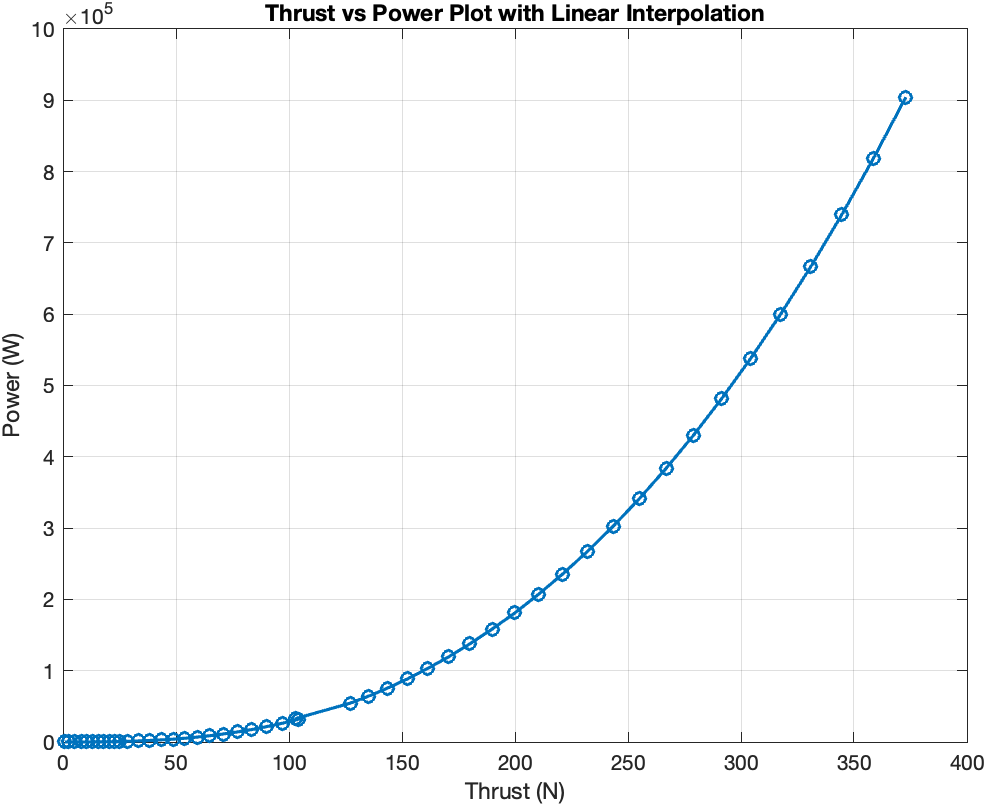
\includegraphics[width=0.5\linewidth]{Linear Interpolation Thrust vs Power.png}
    \caption{Free body diagram}
    \label{fig:Thrust vs Power Graph}
\end{figure}

\FloatBarrier % Enforce placement of floats up to this point

By matching the predicted power at a given thrust to the speed associated with that thrust, a comprehensive Speed vs. Power predictive chart was generated.

By matching the predicted power at a given thrust to the speed associated with that thrust, a comprehensive Speed vs. Power predictive chart was generated.
\begin{figure}[h!]
    \centering
    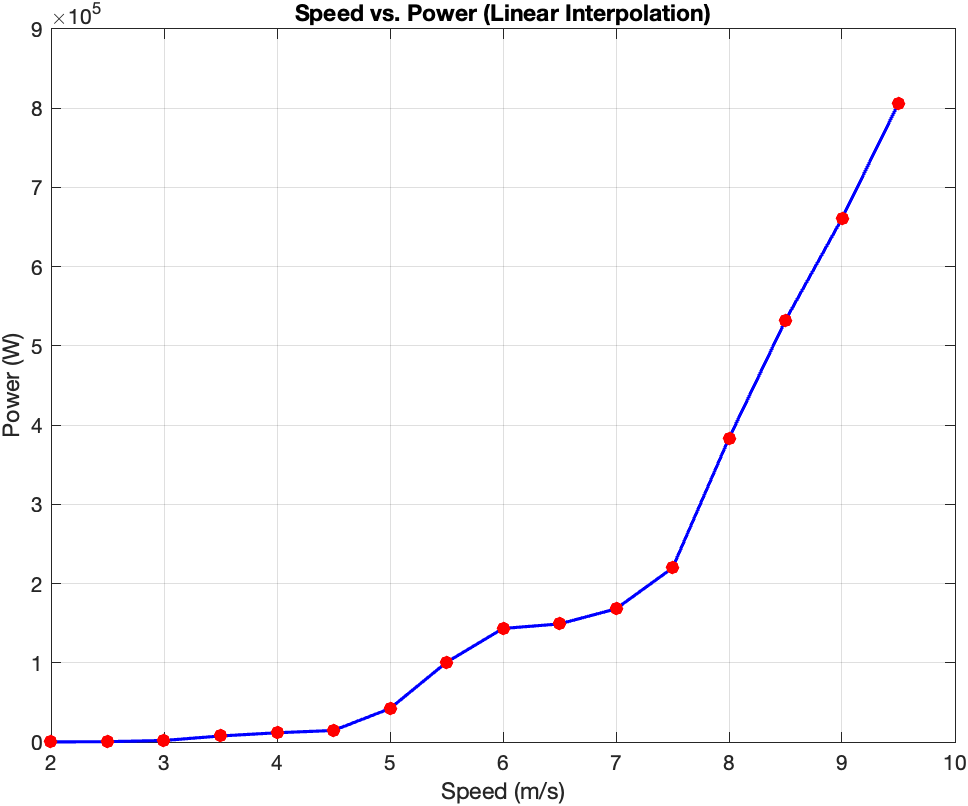
\includegraphics[width=0.5\linewidth]{Linear Interpolation Speed vs Power.png}
    \caption{Free body diagram}
    \label{fig: Speed vs Power Graph}
\end{figure}
The MATLAB-generated Power vs. Speed chart successfully matched power values to the appropriate speeds. The analysis showed that power and speed have a nonlinear relationship, best described by a polynomial fit.


\section{Discussion}
Based on the constraints provided by the power sub-team, the simulations need to be narrowed down to focus on power outputs within the range of 0 to 5000 Watts to improve approximation accuracy.

The results of the simulations and calculations provide insights into the power-speed relationship of the boat. The power requirements at various speeds are obtained through a combination of linear interpolation of experimental drag data and CFD analysis of propeller performance.

The findings from this study can be used to optimize the propeller design and improve the efficiency of the CMUSR boat, ultimately enhancing its performance in the solar-powered boat racing competition.

\section{Conclusion}
This project successfully developed a Power vs. Speed chart using linear interpolation and machine learning techniques. Future work will involve refining the simulations and improving prediction accuracy within the specified power output range.

% Add references here if needed.

\end{document}